\documentclass[]{book}
\usepackage{lmodern}
\usepackage{amssymb,amsmath}
\usepackage{ifxetex,ifluatex}
\usepackage{fixltx2e} % provides \textsubscript
\ifnum 0\ifxetex 1\fi\ifluatex 1\fi=0 % if pdftex
  \usepackage[T1]{fontenc}
  \usepackage[utf8]{inputenc}
\else % if luatex or xelatex
  \ifxetex
    \usepackage{mathspec}
  \else
    \usepackage{fontspec}
  \fi
  \defaultfontfeatures{Ligatures=TeX,Scale=MatchLowercase}
\fi
% use upquote if available, for straight quotes in verbatim environments
\IfFileExists{upquote.sty}{\usepackage{upquote}}{}
% use microtype if available
\IfFileExists{microtype.sty}{%
\usepackage{microtype}
\UseMicrotypeSet[protrusion]{basicmath} % disable protrusion for tt fonts
}{}
\usepackage[margin=1in]{geometry}
\usepackage{hyperref}
\hypersetup{unicode=true,
            pdftitle={Mathe fürs Berufliches Gymnasium sozialwissenschaftliche Richtung (SGGS)},
            pdfauthor={Uwe Sterr},
            pdfborder={0 0 0},
            breaklinks=true}
\urlstyle{same}  % don't use monospace font for urls
\usepackage{natbib}
\bibliographystyle{apalike}
\usepackage{longtable,booktabs}
\usepackage{graphicx,grffile}
\makeatletter
\def\maxwidth{\ifdim\Gin@nat@width>\linewidth\linewidth\else\Gin@nat@width\fi}
\def\maxheight{\ifdim\Gin@nat@height>\textheight\textheight\else\Gin@nat@height\fi}
\makeatother
% Scale images if necessary, so that they will not overflow the page
% margins by default, and it is still possible to overwrite the defaults
% using explicit options in \includegraphics[width, height, ...]{}
\setkeys{Gin}{width=\maxwidth,height=\maxheight,keepaspectratio}
\IfFileExists{parskip.sty}{%
\usepackage{parskip}
}{% else
\setlength{\parindent}{0pt}
\setlength{\parskip}{6pt plus 2pt minus 1pt}
}
\setlength{\emergencystretch}{3em}  % prevent overfull lines
\providecommand{\tightlist}{%
  \setlength{\itemsep}{0pt}\setlength{\parskip}{0pt}}
\setcounter{secnumdepth}{5}
% Redefines (sub)paragraphs to behave more like sections
\ifx\paragraph\undefined\else
\let\oldparagraph\paragraph
\renewcommand{\paragraph}[1]{\oldparagraph{#1}\mbox{}}
\fi
\ifx\subparagraph\undefined\else
\let\oldsubparagraph\subparagraph
\renewcommand{\subparagraph}[1]{\oldsubparagraph{#1}\mbox{}}
\fi

%%% Use protect on footnotes to avoid problems with footnotes in titles
\let\rmarkdownfootnote\footnote%
\def\footnote{\protect\rmarkdownfootnote}

%%% Change title format to be more compact
\usepackage{titling}

% Create subtitle command for use in maketitle
\newcommand{\subtitle}[1]{
  \posttitle{
    \begin{center}\large#1\end{center}
    }
}

\setlength{\droptitle}{-2em}

  \title{Mathe fürs Berufliches Gymnasium sozialwissenschaftliche Richtung (SGGS)}
    \pretitle{\vspace{\droptitle}\centering\huge}
  \posttitle{\par}
    \author{Uwe Sterr}
    \preauthor{\centering\large\emph}
  \postauthor{\par}
      \predate{\centering\large\emph}
  \postdate{\par}
    \date{2019-01-08}

\usepackage{booktabs}

\begin{document}
\maketitle

{
\setcounter{tocdepth}{1}
\tableofcontents
}
\chapter{Handhabung}\label{handhabung}

Diese Dokument ist eine erweiterte Formelsammlung mit Beispielen und
soll bei der Lösung von Aufgaben und bei der Klausurvorbereitung helfen.
Es ist abzuwägen ob es aufgrund der verfügbaren elektronischen
Hilfsmittel eine papierbasierte Formelsammlung noch geeignet ist.

\chapter{Mengenlehre}\label{intro}

Hier werden Schreibweisen von Mengen und die Einteilung von reelen
Zahlen eingeführt

\section{Einteilung von reelen
Zahlen}\label{einteilung-von-reelen-zahlen}

\subsection{Rationale Zahlen}\label{rationale-zahlen}

\[\mathbb { Q } = \left\{ \ldots , - \frac { 2 } { 1 } , - \frac { 1 } { 2 } , - \frac { 1 } { 1 } , 0 , \frac { 1 } { 1 } , \frac { 1 } { 2 } , \frac { 2 } { 1 } , \frac { 1 } { 3 } , \ldots \right\} = \left\{ \frac { p } { q } | p \in \mathbb { Z } , q \in \mathbb { N } \backslash \{ 0 \} \right\}\]

\subsection{Ganze Zahlen}\label{ganze-zahlen}

\[\mathbb { Z } = \{ \ldots , - 2 , - 1,0,1,2 , \ldots \}\]

\subsection{Natürliche Zahlen}\label{naturliche-zahlen}

\[\mathbb { N } ( \text { ohne } 0 ) : \{ 1,2,3 , \ldots \} \text { oder (mit } 0 ) : \{ 0,1,2,3 , \ldots \} \left( \text { auch } \mathbb { N } _ { 0 } \right)\]

\section{Notation für häufig verwendete Teilmengen der reellen
Zahlen}\label{notation-fur-haufig-verwendete-teilmengen-der-reellen-zahlen}

\url{https://www.mathebibel.de/mengenlehre}

Die Menge aller reellen Zahlen\\
- außer der Zahl a: \textbf{\(\mathbb { R } \backslash \{ a \}\)}\\
- größer gleich a: \(\{ x \in \mathbb { R } | x \geq a \}\)\\
- Die Menge A besteht aus den Elementen x für die gilt
\(A = \{ x | - 5 < x < 3 \}\)

\chapter{Funktionen}\label{funktionen}

Beispiele und Merkmal von Funktionen

\section{Grenzwert}\label{grenzwert}

\url{https://de.wikipedia.org/wiki/Grenzwert_(Funktion)}

\(\lim _ { x \rightarrow 0 } \left( \frac { 1 } { x } \right) = + \infty\)

\section{Verschiebung}\label{verschiebung}

Durch addition von Werten zu den jeweiligen x und y Werten wird die
Orginalfunktion in der jeweiligen Richtung verschoben. Es gilt:

Um einen Funktionsgraph in y-Richtung zu verschieben, muss man eine Zahl
a zum Funktionsterm addieren oder subtrahieren.

Eine Verschiebung in x-Richtung erreicht man, indem man x durch x+a oder
x−a ersetzt.

Ein weiters Beispiel für eine Funktionsverschiebung ist in Bild
\ref{fig:funk2} für die Funktion \(x^2+2*x+3\) dargestellt

\begin{figure}
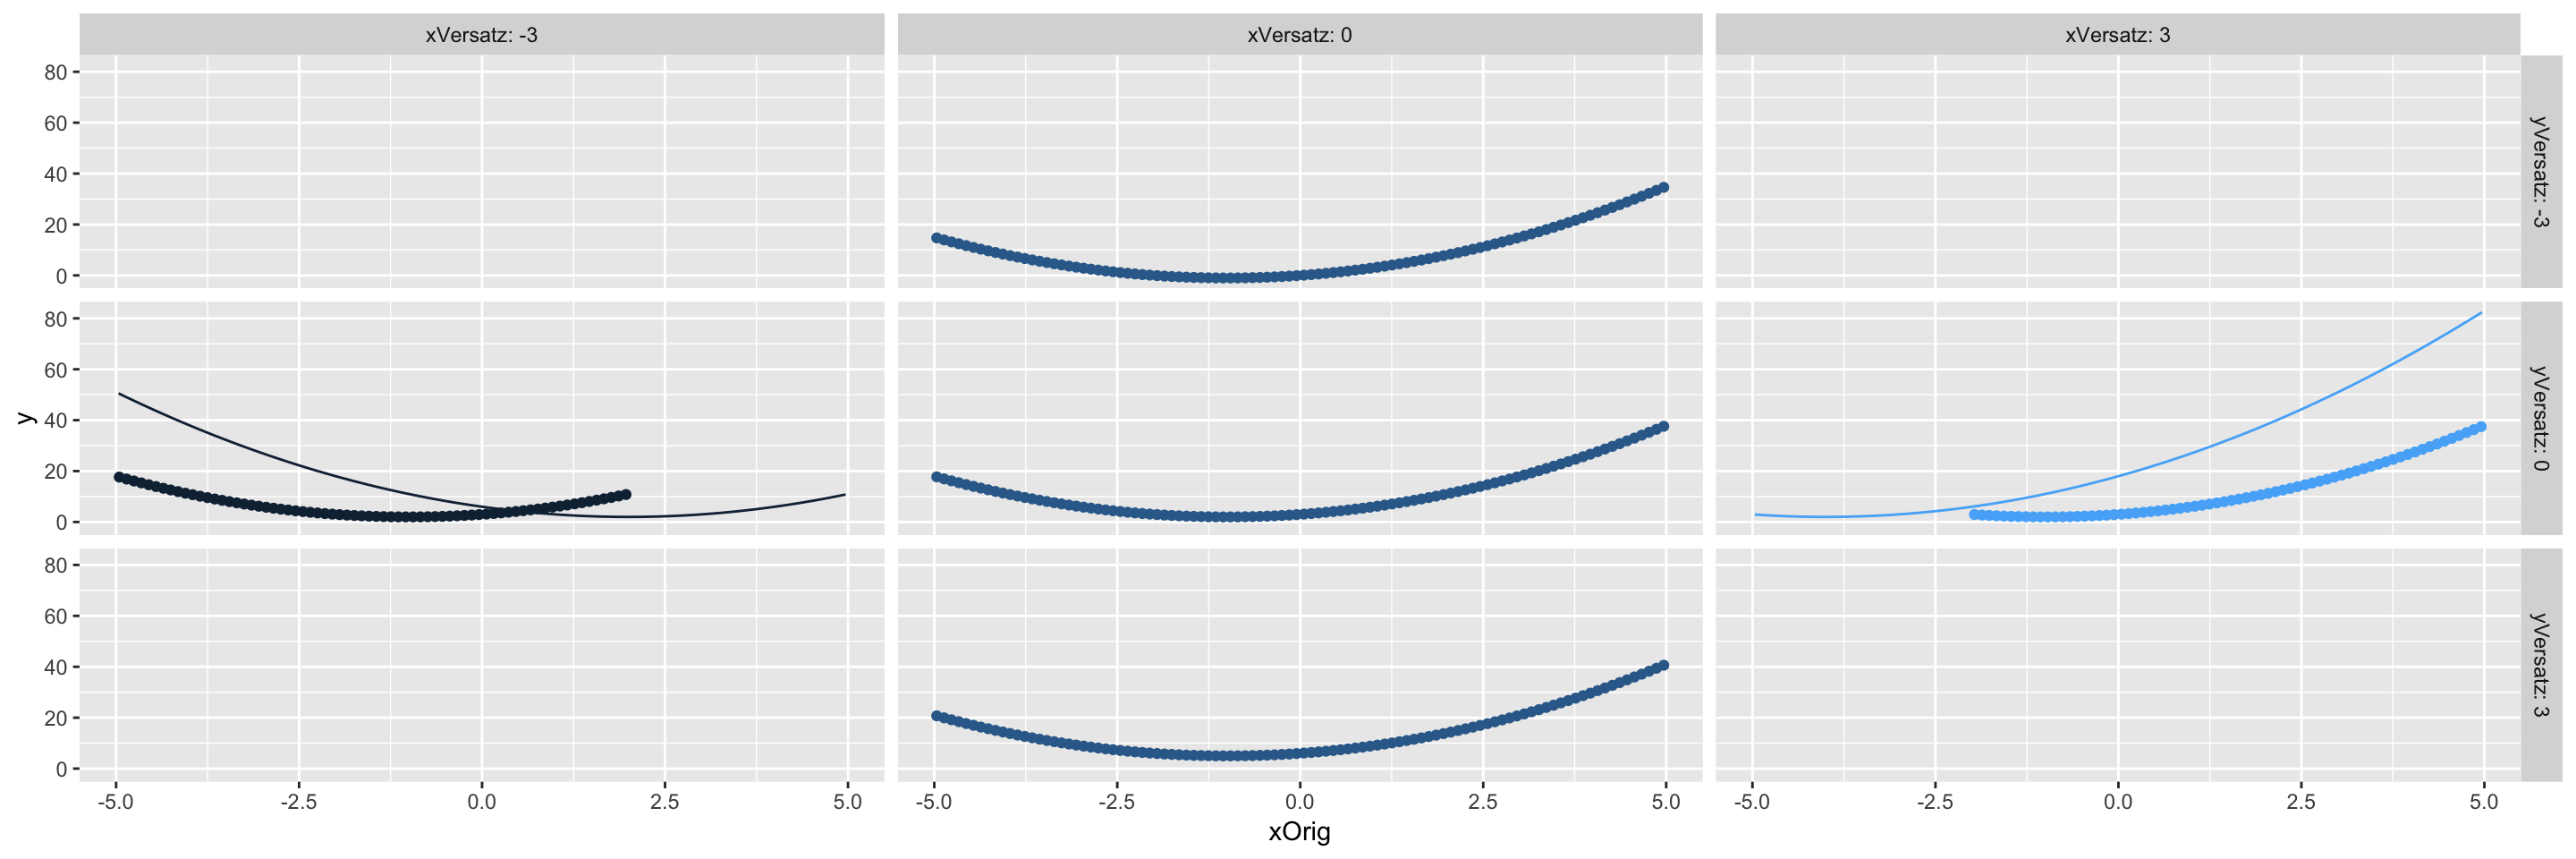
\includegraphics[width=1.6\linewidth]{RFormelSammlung_files/figure-latex/funk2-1} \caption{Funktion $x^2+2*x+3$ verschoben}\label{fig:funk2}
\end{figure}

\section{Stauchung}\label{stauchung}

In Bild \ref{fig:funk3} wird in der Orginalfunktion sowohl x als auch y
multipliziert. Die Orginalfunktion ist in der Mitte der Plots.

\begin{figure}
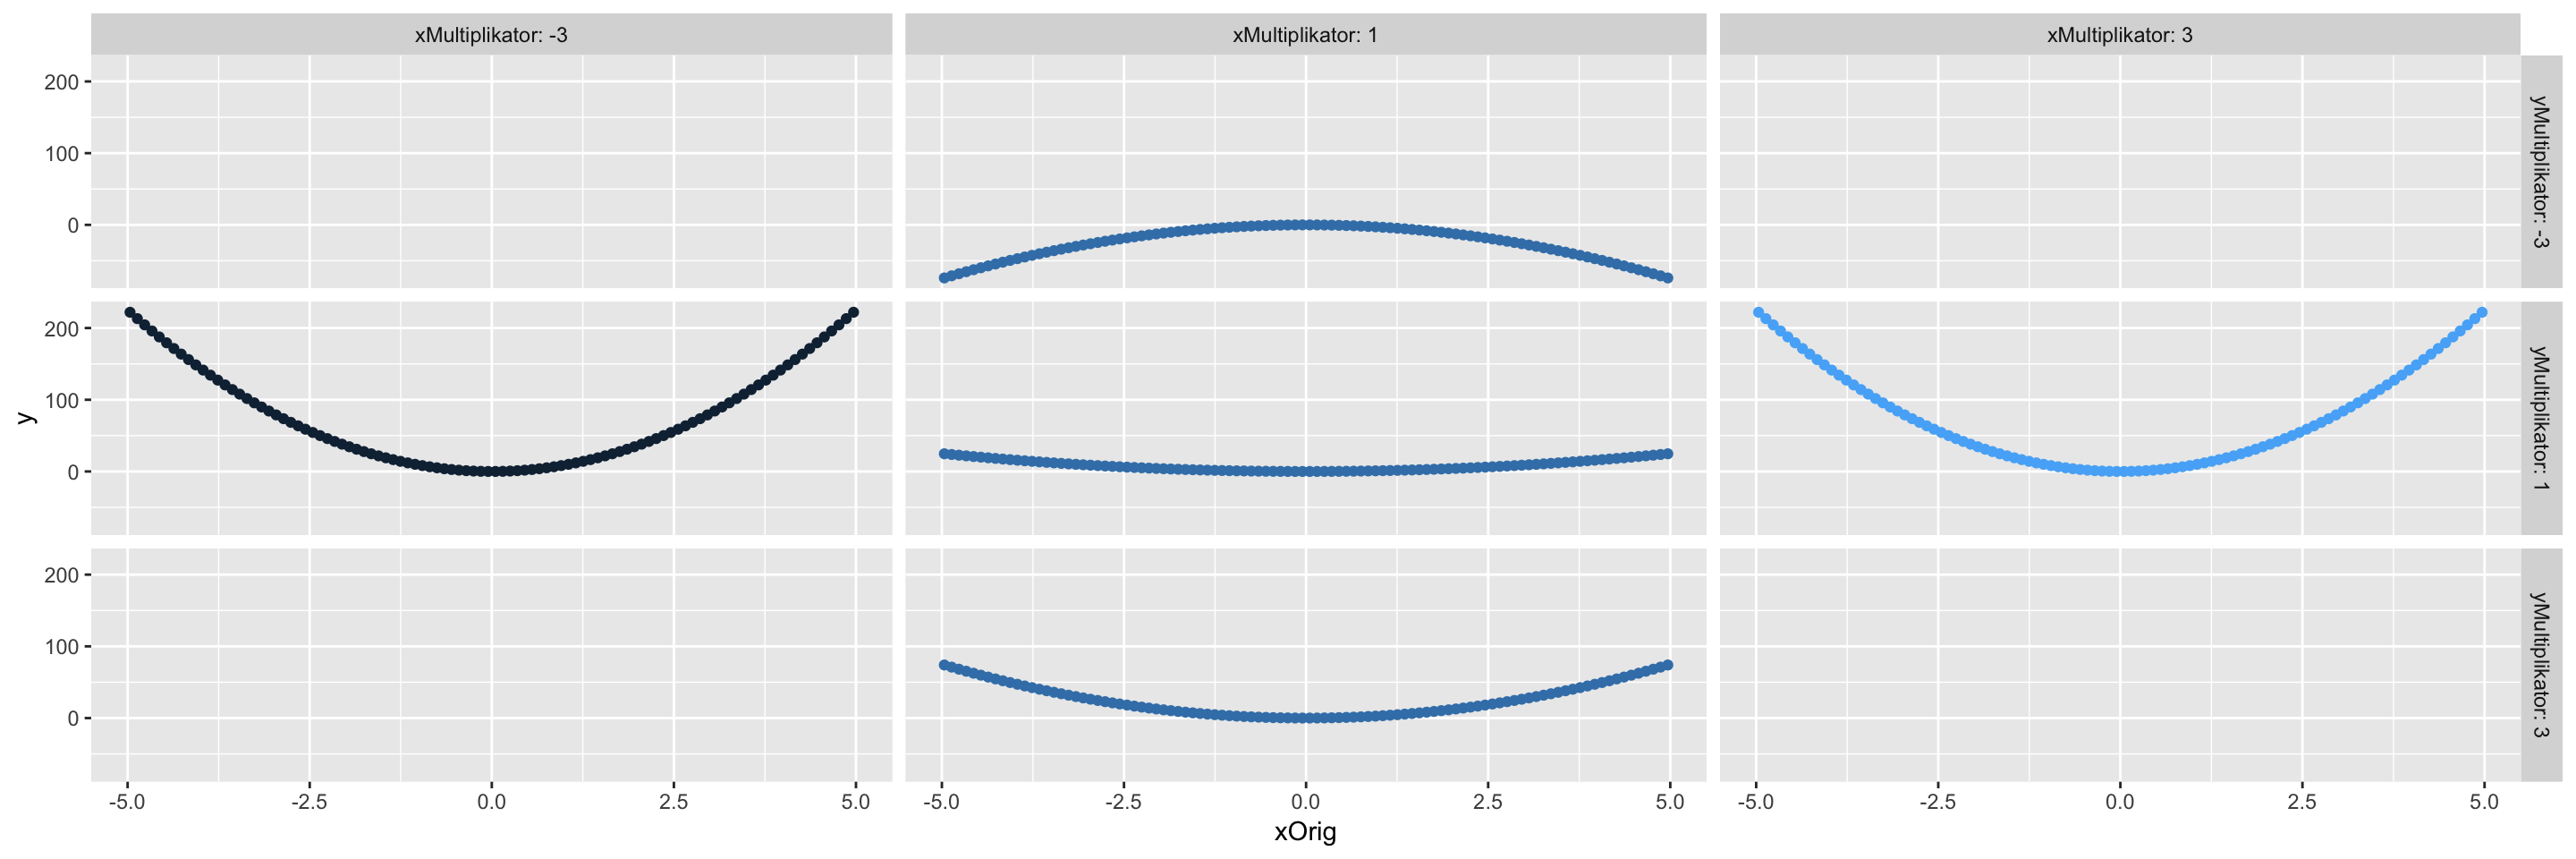
\includegraphics[width=1.6\linewidth]{RFormelSammlung_files/figure-latex/funk3-1} \caption{Funktion in x und y gestreckt und gestaucht}\label{fig:funk3}
\end{figure}

Siehe nachfolgende Mind Map als Gedankenstütze

\begin{figure}

{\centering 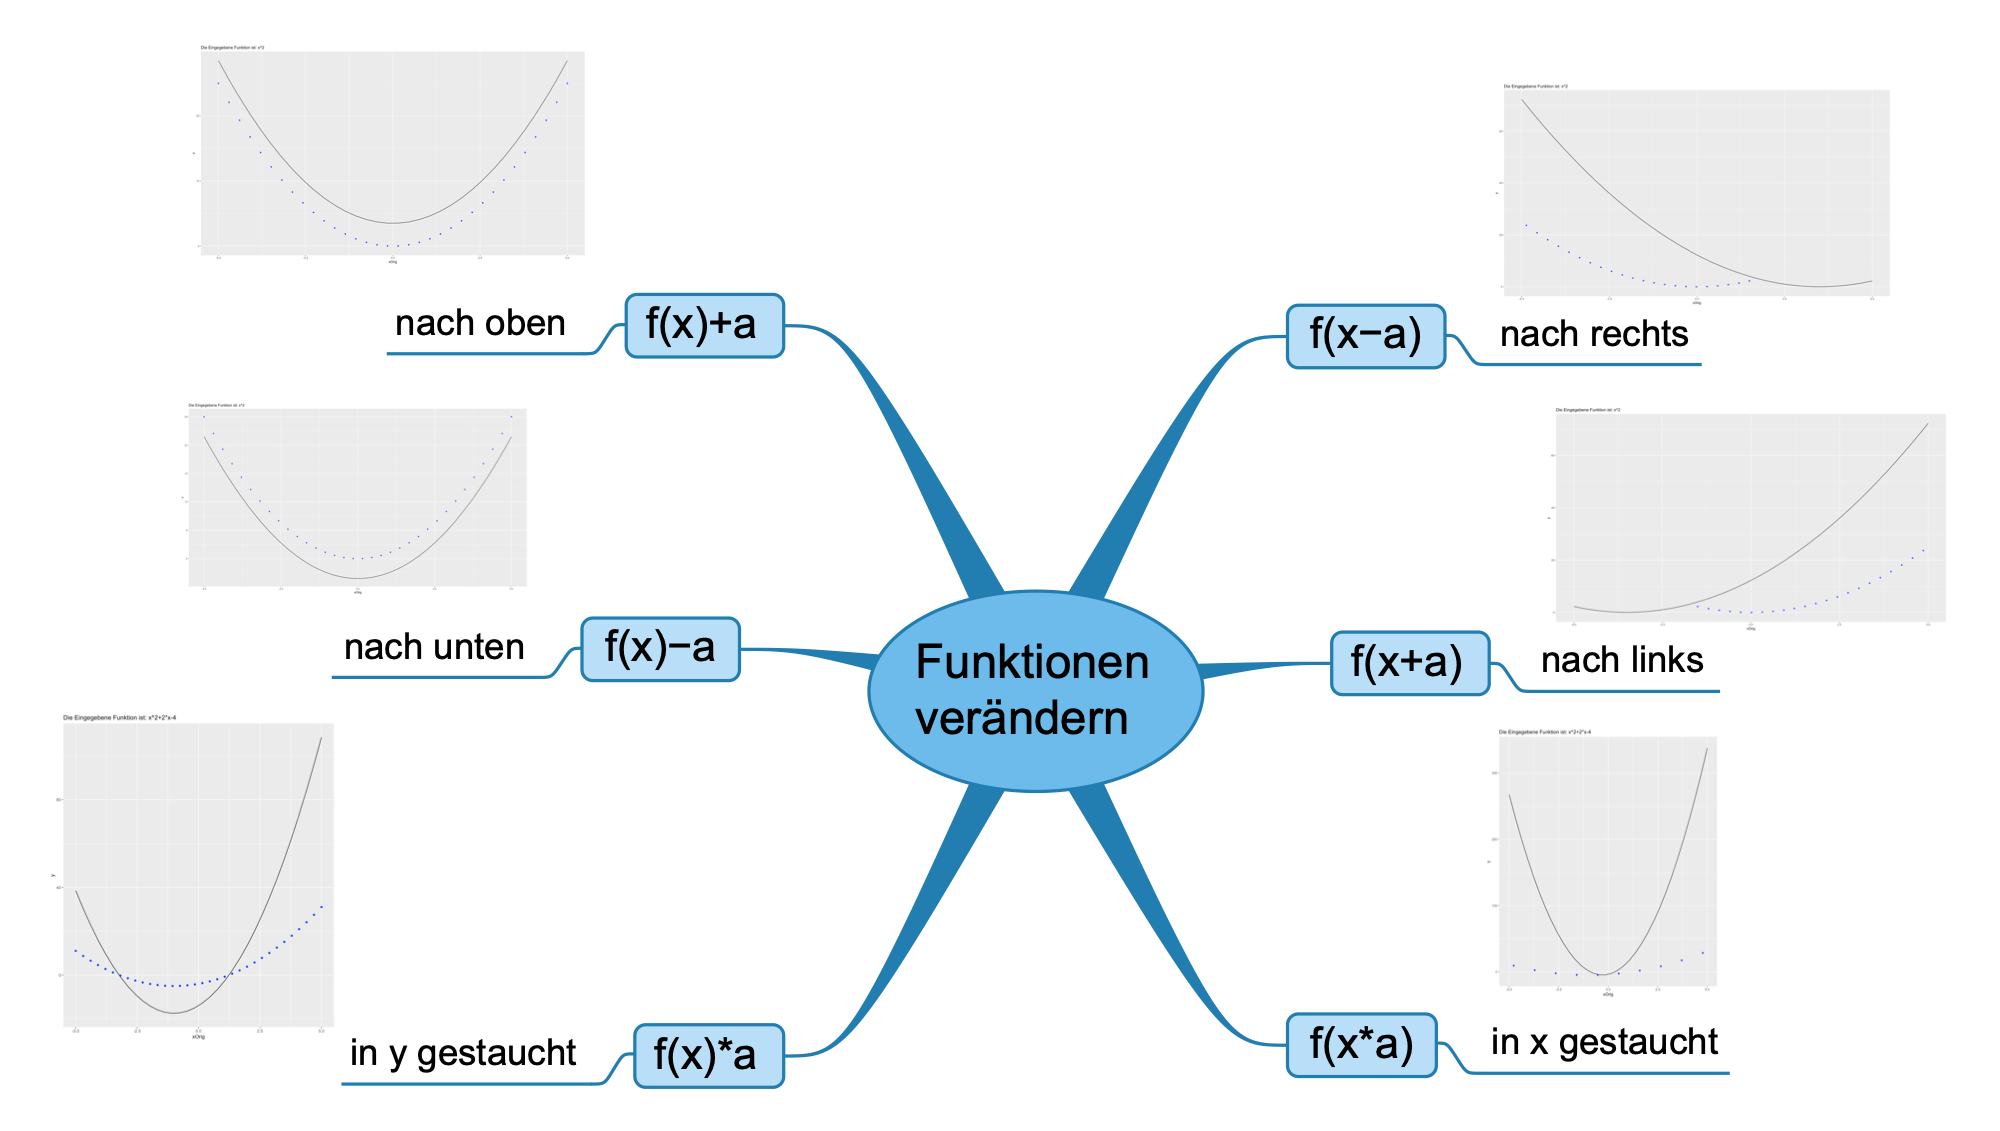
\includegraphics[width=25in]{image/FunktionsVerschiebung} 

}

\caption{Verschiebung durch addtion}\label{fig:mindMapVerschiebung}
\end{figure}

\bibliography{book.bib,packages.bib}


\end{document}
